\chapter{Code Description and Developer Guidelines}
\label{chap-dev}

\renewcommand{\headrulewidth}{0.3pt}
\fancyhead[LE]{\thepage} \fancyhead[RE]{\nouppercase{\textbf{\leftmark}}}
\fancyhead[RO]{\thepage} \fancyhead[LO]{\nouppercase{\textbf{\rightmark}}}
\fancyfoot[L,C,R]{}

\setlength{\parindent}{0.35cm}

\minitoc
\newpage
% ================================================================

This chapter first describes the conceptual architecture --- the HTAS/CWV split and the three backend layers (\cref{chap-description-src}) --- then states the \textbf{rules} a developer must follow when working within that structure, and the concrete recipes for extending the application.

\section{Code Description}
\label{chap-description-src}

\cwv~is built on top of a standalone scientific backend and consumes it through a well-defined public interface. Understanding the code therefore means understanding two things: how the QGIS application and the backend are kept \emph{separate}, and how the backend is internally organised into \emph{three layers}. This section describes both; the strict rules a developer must follow when working within this structure are collected in the remainder of this chapter.

\subsection{Split Architecture: HTAS and CWV}
\label{sec-split}

\cwv~is maintained as two packages that are kept \textbf{strictly independent}:

\begin{itemize}
    \item \textbf{\script{HydrologicalTwinAlphaSeries} (HTAS)} --- the standalone scientific backend: simulation processing, domain structures (compartments, meshes, observations), configuration models, and the \script{HydrologicalTwin} facade. It lives under \script{external/HydrologicalTwinAlphaSeries}; in the published setup this path is a \gitlab~submodule pointing to the standalone backend repository.
    \item \textbf{\script{cawaqsviz} (CWV)} --- the standalone QGIS application: dialog boxes, visualisation workflows, GIS integration, and application-side adapters.
\end{itemize}

Independence is a hard architectural constraint, not a style preference:

\begin{itemize}
    \item HTAS must not depend on QGIS, \script{Qt}, dialog code, or any \cwv~frontend module;
    \item \cwv~must consume HTAS through its public API and keep QGIS-specific adaptation code on the application side. Runtime HTAS imports belong in \script{interface/}; \script{frontend/} modules access backend behaviour only through the application gateway;
    \item synchronisation between the two repositories happens through version control and dependency pinning, not through code duplication.
\end{itemize}

\begin{landscape}
    \begin{figure}[p]
        \centering
        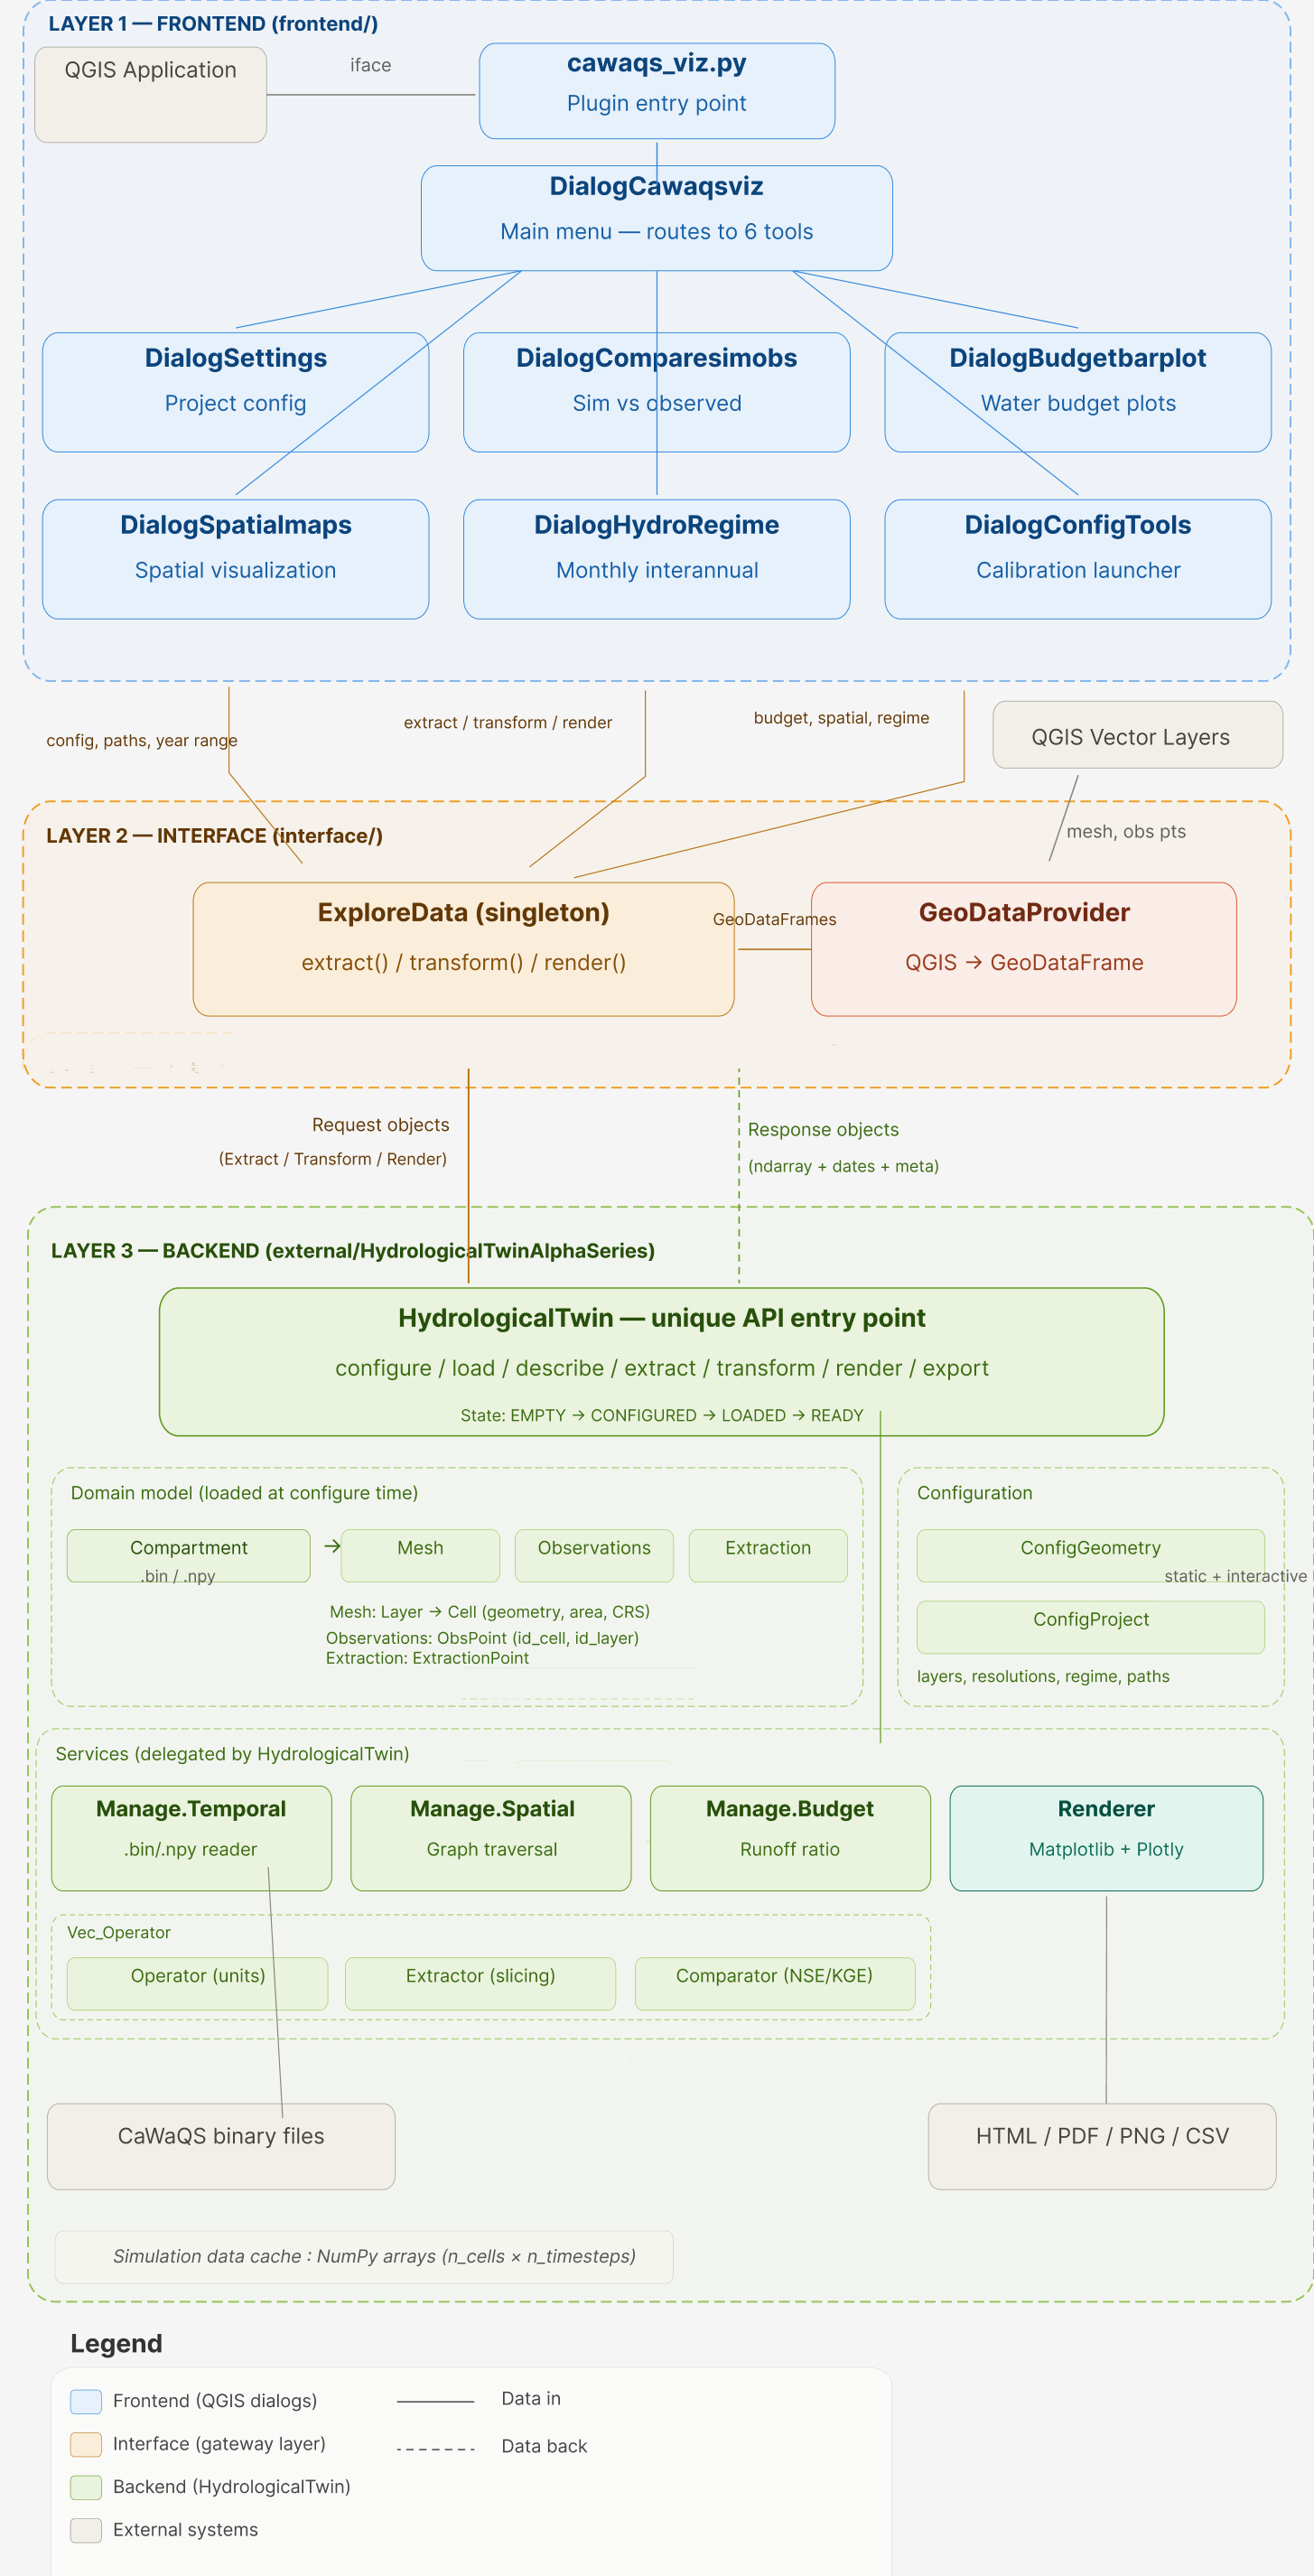
\includegraphics[width=\linewidth,height=0.85\textheight,keepaspectratio]{5_develloppeur/fig/architecture_developer_overview.png}
        \caption{\cwv~+~HTAS architecture --- detailed component diagram with data flow (CWV HTAS in Aril 2026). NB: the 3 layers the image refer to are not the same ones were mentioned above!}
        \label{fig-architecture-overview}
    \end{figure}
\end{landscape}

\subsection{The Three Layers of the Backend}
\label{sec-layers}

HTAS is organised as a \textbf{three-level architecture} in which each level may call the level below it, never the level above. Each level has one canonical entry module, and imports point \textbf{strictly downward} (L1~$\rightarrow$~L2~$\rightarrow$~L3): never up, never sideways within a level. Because every dependency points downward, the layers can never form an import loop --- the dependency graph is acyclic.

\begin{lstlisting}[language=bash, caption={The three backend layers and their canonical entry modules.}, label={code-layers}]
L1 - HT CLIENT - MACRO        ht/client/hydrological_twin_client.py       (may import L2, L3)
L2 - HT DEVELOPER - MICRO     ht/developer/hydrological_twin_developer.py (may import L3)
L3 - SERVICES - ELEMENTARIES  services/                                   (imports nothing in ht/)
\end{lstlisting}

Taken together with the QGIS-side layers (frontend and interface), the roles are summarised in \cref{tab-layers}.

\renewcommand{\arraystretch}{1.3}
\begin{table}[H]
    \centering
    \begin{tabularx}{\linewidth}{>{\raggedright\arraybackslash}m{3.6cm}|X}
        \hline
        \textbf{Layer} & \textbf{Role} \\
        \hline
        \textbf{Frontend} \newline \script{frontend/} & QGIS dialog boxes. They own user interaction and route a single coarse call per workflow to the interface. \script{Qt}/\script{PyQt5} lives here and only here. \\
        \hline
        \textbf{Interface} \newline \script{interface/} & \script{ExploreData} is the \textbf{only} gateway to the backend; \script{GeoDataProvider} turns QGIS vector layers into \script{GeoDataFrame}s so the backend stays QGIS-agnostic. \\
        \hline
        \textbf{L1 - HT CLIENT - MACRO} \newline \script{ht/client/} & \script{HydrologicalTwinClient} exposes one method per user-facing dialog operation. Each delegates to a matching \script{operations\_client.run\_*} that owns the full \script{fetch}~$\rightarrow$~\script{transform}~$\rightarrow$~\script{render} chain and returns a typed \script{*Result} dataclass. Zero \script{qgis}/\script{PyQt5} imports --- usable from a notebook today, from an HTTP server tomorrow. \\
        \hline
        \textbf{L2 - HT DEVELOPER - MICRO} \newline \script{ht/developer/} & \script{HydrologicalTwin} is the micro-verb facade exposing 8 canonical verbs with an explicit \script{EMPTY}~$\rightarrow$~\script{CONFIGURED}~$\rightarrow$~\script{LOADED}~$\rightarrow$~\script{READY} state machine. Useful for notebook exploration and for operations not yet promoted to the client. \\
        \hline
        \textbf{L3 - SERVICES - ELEMENTARIES} \newline \script{services/} & Finest-grained computations and I/O: operators, renderer, twin-state reads and disk-cache provisioning (\script{twin\_io.py}), and leaf data DTOs (\script{io\_types.py}). No module under \script{services/} imports from \script{ht/} --- the import graph is a strictly downward, acyclic DAG. \\
        \hline
    \end{tabularx}
    \caption{Roles of the frontend, interface, and the three backend layers.}
    \label{tab-layers}
\end{table}

\script{ExploreData} calls \textbf{the client} for coarse operations (the normal path) and can still reach the developer twin \textit{via} \script{client.\_twin} for low-level micro-verb calls. A more annotated view of the data flow is given in \cref{fig-architecture-overview}.

\subsection{Example Workflow: the Budget Bar Plot}
\label{sec-example-workflow}

The following walk-through shows what happens, step by step, when a user creates a water budget bar plot. It is one of the most complete workflows, chaining \script{fetch}~$\rightarrow$~\script{transform}~$\rightarrow$~\script{render}, and it is useful for understanding the number of round-trips between layers --- especially when designing the future server API.

\begin{enumerate}
    \item In the \script{DialogBudgetbarplot} dialog box, the user selects variables, a period, a frequency, and an aggregation.
    \item The dialog issues a \emph{single} coarse call to \script{ExploreData}, which forwards it to \script{HydrologicalTwinClient.budget\_barplot(**kwargs)}, which in turn calls \script{operations\_client.run\_budget\_barplot}.
    \item For each variable (rain, ETR, infiltration, runoff), the orchestration calls \script{twin.fetch} (reads the simulation matrix from disk through the services layer) then \script{twin.transform} (spatial mean + temporal aggregation).
    \item A final \script{twin.render} call produces the plot; the renderer writes a PNG and a CSV to disk and returns their paths.
    \item The paths are bundled into a \script{BudgetBarplotResult} dataclass and returned up the chain to the dialog, which opens the plot file.
\end{enumerate}

What this reveals for API design:

\begin{itemize}
    \item today, everything between \script{ExploreData} and the developer twin is \textbf{in-process}. The natural network seam is the \script{ExploreData}~$\rightarrow$~\script{Client} boundary, not \script{ExploreData}~$\rightarrow$~\script{HydrologicalTwin};
    \item \textbf{one coarse operation = one server round-trip}. The dialog calls \script{client.budget\_barplot(...)} once; the inner loop of 4 fetches + 4 transforms + 1 render stays server-side inside \script{run\_budget\_barplot}. The former ``9-calls-per-plot'' cost collapses to a single call at the network boundary;
    \item \textbf{the client \emph{is} the future HTTP surface.} Each \script{HydrologicalTwinClient} method maps cleanly to one endpoint, with a typed \script{*Result} dataclass as the response schema. The developer micro-verb API stays available for notebook-style exploration;
    \item \textbf{rendering still writes to disk.} When the client moves server-side, render outputs will need to return data (or signed URLs) instead of local file paths --- the \script{*Result} dataclasses are the right place to evolve that contract.
\end{itemize}

\subsection{Key Properties}
\label{sec-key-properties}

\begin{itemize}
    \item the \textbf{interface layer} is the cut point for a future server deployment --- everything below it could run remotely;
    \item the backend \textbf{never imports} QGIS or \script{Qt} (enforced by CI);
    \item all backend calls use \textbf{Request/Response objects} (e.g. \script{ExtractRequest}~$\rightarrow$~\script{ExtractValuesResponse});
    \item the \script{HydrologicalTwin} follows a \textbf{state machine} lifecycle: \script{EMPTY}~$\rightarrow$~\script{CONFIGURED}~$\rightarrow$~\script{LOADED}~$\rightarrow$~\script{READY}.
\end{itemize}

\section{Architectural Rules}
\label{sec-dev-rules}

\subsection{The hard rule: QGIS lives in the frontend only}

\cwv~is split into two packages that are kept \textbf{strictly independent}: the \script{HydrologicalTwinAlphaSeries} (HTAS) scientific backend under \script{external/HydrologicalTwinAlphaSeries}, and the \script{cawaqsviz} (CWV) QGIS application on top of it. The separation is an \textbf{architectural invariant}:

\begin{itemize}
    \item HTAS must \textbf{never} import \script{qgis.*}, \script{PyQt5}, \script{processing}, or anything from \script{cawaqsviz/}. If you are about to add such an import inside \script{external/HydrologicalTwinAlphaSeries/}, stop --- the work belongs on the CWV side;
    \item CWV consumes HTAS only through its public API (the two entry gates, \cref{sec-dev-gates});
    \item the backend is designed to be \textbf{usable from a notebook today and a server tomorrow} (\cref{sec-notebook-usage}). Anything that breaks notebook-from-pure-Python usage also breaks the future server.
\end{itemize}

\subsection{The three-layer target structure}

HTAS is a three-level layered architecture (\cref{sec-layers}): each level may call the level below it, never the level above.

\begin{lstlisting}[language=bash, caption={Canonical entry modules per layer; imports point strictly downward.}, label={code-layers-dev}]
L1 - HT CLIENT - MACRO        ht/client/hydrological_twin_client.py       (may import L2, L3)
L2 - HT DEVELOPER - MICRO     ht/developer/hydrological_twin_developer.py (may import L3)
L3 - SERVICES - ELEMENTARIES  services/                                   (imports nothing in ht/)
\end{lstlisting}

\textbf{Golden rule --- imports point downward only.} Never up, never sideways within a level. No module under \script{services/} may import from \script{ht/client/} or \script{ht/developer/}. Shared data DTOs live at the L3 leaf (\script{services/public/io\_types.py}) and are re-exported by the L2 \script{api\_types.py}, so the edge stays downward. Because every dependency points downward, the graph can never form an import loop.

\textbf{Golden rule (corollary) --- L1 only orchestrates, it does not handle data.} L1 (\script{hydrological\_twin\_client.py} and, behind it, \script{operations\_client.py}) is \emph{pure orchestration}: it may only \emph{call} L2 micro-verbs and \emph{bundle} their typed results into a \script{*Result} dataclass. It must contain \textbf{no data handling of its own} --- no \script{DataFrame} construction, no array reshaping or aggregation, no unit/path/provenance shaping, no disk I/O, no domain computation. Any such logic belongs \emph{down} in an L2 micro-verb (\script{fetch}/\script{transform}/\script{render}/\script{export}, or a new \script{kind=}) or in L3 \script{services/}. The test: if a line in \script{ht/client/} does anything other than call a lower layer or pack/unpack a typed result, it is in the wrong layer.

\alertwarning{The code is honest about being in transition: the clean single L2~$\rightarrow$~L3 arrow described here is the \emph{target}, not yet the literal code. See the current-state caveats below.}

\noindent Two current-state caveats a developer must keep in mind:
\begin{itemize}
    \item inside L2, \script{ht/developer/dispatch.py} and \script{ht/developer/handlers.py} are \textbf{transitional} L2-internal modules. Today the micro-verbs route \script{hydrological\_twin\_developer.py}~$\rightarrow$~\script{dispatch.py}~$\rightarrow$~\script{handlers.py} before reaching L3; these two modules are slated to be folded into the L2 micro-verb bodies (see \script{external/HydrologicalTwinAlphaSeries/docs/TODO.md});
    \item a few downward imports across layers (e.g. reuse of the fetch-simulation-matrix function inside several L2 methods) are tolerated for now and will be tightened later. They do not currently pose problems for notebook usage.
\end{itemize}

\section{Entry Gates}
\label{sec-dev-gates}

All frontend~$\rightarrow$~backend calls go through one of two surfaces. Do not reach around them.

\subsection{Client gate --- L1 - HT CLIENT - MACRO}

\script{HydrologicalTwinClient} (\script{ht/client/hydrological\_twin\_client.py}) exposes \textbf{one method per user-facing dialog operation}:

\begin{itemize}
    \item \script{budget\_barplot}, \script{hydrological\_regime};
    \item \script{spatial\_map\_watbal}, \script{spatial\_map\_aq};
    \item \script{compare\_sim\_obs}, \script{statistical\_criteria};
    \item \script{mask\_watbal}, \script{mask\_hyd\_boundary}, \script{mask\_aq\_boundary}.
\end{itemize}

Plus the lifecycle methods \script{configure}, \script{load}, \script{describe}, \script{is\_ready}, and the one-shot \script{build} classmethod. Each operation wraps a full \script{fetch}~$\rightarrow$~\script{transform}~$\rightarrow$~\script{render} chain server-side and returns a typed \script{*Result} dataclass (defined in \script{ht/client/api\_types.py}, orchestrated by \script{ht/client/operations\_client.py}). \textbf{This is the surface a future HTTP server will expose:} one coarse operation = one round-trip. Frontend dialogs should prefer this gate.

\subsection{Developer gate --- L2 - HT DEVELOPER - MICRO}

\script{HydrologicalTwin} (\script{ht/developer/hydrological\_twin\_developer.py}) exposes the 8 canonical verbs:

\begin{itemize}
    \item lifecycle (inline): \script{configure}, \script{load}, \script{describe}, \script{export};
    \item dispatching (routed by \script{kind=} through the transitional \script{dispatch.py}~$\rightarrow$~\script{handlers.py}, then down to L3): \script{fetch}, \script{mask}, \script{transform}, \script{render}.
\end{itemize}

State machine: \script{EMPTY}~$\rightarrow$~\script{CONFIGURED}~$\rightarrow$~\script{LOADED}~$\rightarrow$~\script{READY}. Each verb checks the state via \script{\_require\_state} and raises \script{InvalidStateError} if called too early. The developer gate is the \textbf{power-user / notebook / exploration} surface. Use it for operations not yet promoted to the client, and for low-level work; \script{ExploreData} can still reach it \textit{via} \script{client.\_twin} when needed.

\section{Adding a New Dialog Operation}
\label{sec-dev-add-op}

To add a new dialog-level workflow, follow three steps:

\begin{enumerate}
    \item define a \script{*Result} dataclass in \script{ht/client/api\_types.py};
    \item implement \script{run\_<name>} in \script{ht/client/operations\_client.py} --- it owns the \script{fetch}~$\rightarrow$~\script{transform}~$\rightarrow$~\script{render} orchestration;
    \item add a one-line facade method on \script{HydrologicalTwinClient}, then call it from \script{ExploreData}.
\end{enumerate}

Method bodies on the client class are intentionally thin ($\leq$~5 statements). Keep them that way.

\section{When Editing --- Checklist}
\label{sec-dev-checklist}

\begin{itemize}
    \item touching dialog code? $\rightarrow$ \script{frontend/Dialog*.py}. Route through \script{ExploreData};
    \item adding a new dialog-level workflow? $\rightarrow$ the three-step recipe above (\cref{sec-dev-add-op});
    \item adding a new compute primitive? $\rightarrow$ \script{ht/developer/handlers.py} (compute) or \script{services/public/twin\_io.py} (L3 state reads / disk I/O); route \textit{via} \script{dispatch.py} with a new \script{kind=};
    \item found a \script{qgis} / \script{PyQt5} import in \script{external/HydrologicalTwinAlphaSeries/}? $\rightarrow$ bug. Move it to \script{interface/} or \script{frontend/};
    \item found a module under \script{services/} importing from \script{ht/client/} or \script{ht/developer/}? $\rightarrow$ bug. That is an \emph{upward} import; imports must point downward only;
    \item found a frontend module reaching past \script{ExploreData} into HTAS internals? $\rightarrow$ bug. Route through the client gate;
    \item found data handling inside \script{ht/client/} (\script{DataFrame} building, array reshaping/aggregation, unit/path shaping, disk I/O, domain math)? $\rightarrow$ bug. L1 only orchestrates.
\end{itemize}

\section{Conventions}
\label{sec-dev-conventions}

\begin{itemize}
    \item \textbf{Environment:} \script{pixi}-managed (\script{pixi.toml}, \script{pixi.lock}). QGIS, Python, and all dependencies are pinned in a single reproducible environment (\cref{sec-install-pixi});
    \item \textbf{Sync helpers:} \script{./verifState.sh} (diagnostics) and \script{./updateProject.sh} (ordered multi-repository / submodule sync);
    \item \textbf{Pre-lifecycle discovery} (no twin required): \script{HydrologicalTwinClient.detect\_from\_out\_caw(...)} and \script{detect\_project\_neighbors(...)} --- static helpers used by \script{DialogSettings} to auto-fill paths before \script{configure} / \script{load};
    \item \textbf{Compatibility shim:} \script{cawaqsviz/backend}, if present, re-exports HTAS symbols. The real implementation lives only in \script{external/HydrologicalTwinAlphaSeries/}.
\end{itemize}

\section{Version Update}

The plugin version is specified in the \script{metadata.txt} file contained in code excerpt \ref{code_metadata}.
\begin{lstlisting}[language=json, caption={Mandatory information to fill in the \script{metadata.txt} file}, label={code_metadata}]
[general]
name=CaWaQS-Viz
qgisMinimumVersion=3.0
description=Description
version=0.1.16
author=Lise-Marie GIROD (Mines Paris - PSL), Nicolas Flipo (Mines Paris - PSL)
email=lise-marie.girod@minesparis.psl.eu

about=Python QGIS-based vizualization software for CaWaQS3.x

repository=https://gitlab.com/gviz/cawaqsviz
\end{lstlisting}

\section{Code Documentation} 

The code documentation is published on the following link via GitLab Pages: \href{https://cawaqsviz-gviz-adf347ff6d9d45c174db091497a2dfc0f14305cdb4ed9070.gitlab.io/}{https://cawaqsviz-gviz-adf347ff6d9d45c174db091497a2dfc0f14305cdb4ed9070.gitlab.io/}. The documentation is maintained through docstrings in the application modules, following the formatting shown in the example below. 


\begin{lstlisting}[language=Python, caption={Docstring formatting for automatic integration into code documentation}, label={code_format_docstrings}]
class Exemple:
    """
    Resume des fonctionnalites de la classe.
    """

    def __init__(self, arg1):
        """
        Methode constructeur.

        :param arg1: descriptif du parametre
        :type arg1: str
        """
        self.arg1 = arg1

    def do_something(self, arg1: list) -> str:
        """
        Descriptif de la fonction.

        :param arg1: descriptif du parametre
        :type arg1: list
        :return: descriptif de ce que la fonction retourne
        :rtype: str
        """
        return ", ".join(map(str, arg1))
\end{lstlisting}
\vspace{1em}
Compilation is performed by \script{Sphinx}\footnote{whose documentation is accessible via \href{https://www.sphinx-doc.org/en/master/}{https://www.sphinx-doc.org/en/master/}}. The \script{docs/sources} directory contains the configuration files (\script{Conf.py}), as well as the documentation content. 
When integrating new modules into the plugin, adding them to the index (\script{index.rst}) is necessary for the code docstring to appear on the documentation page. This index integrates 3 files: \script{frontend.rst}, \script{interface.rst}, \script{backend.rst}, which contain the classes to be documented. Integrating a new module into the application requires it to be added to these files in the format of code excerpt \ref{code_format_rst}. Updates to the documentation source files must be committed and synchronised with the repositories. 

\begin{lstlisting}[language=Python,caption={Docstring formatting for automatic integration into code documentation}, label={code_format_rst}]
Module
------

.. automodule:: cawaqsviz.Module
   :members:
   :show-inheritance:
   :undoc-members:
\end{lstlisting}

\vspace{1em}

Finally, with each new commit to the \script{Main} or 
\script{Beta} branches, the documentation is compiled according to the content of the \script{docs/source} directory of the repository.

\begin{lstlisting}
image: python:3.9

stages:
  - build
  - deploy

before_script:
  - pip install -U pip
  - pip install -r requirements.txt

build-docs:
  stage: build
  script:
    - sphinx-build -b html docs/source public
  artifacts:
    paths:
      - public

pages:
  stage: deploy
  script:
    - echo "Pages deployed"
  artifacts:
    paths:
      - public
  only:
    - main  
    - beta

\end{lstlisting}

\newpage
\section{Debugging Tools}
\subsection{The \script{Plugin Reloader} plugin}

This utility allows reloading a plugin after a code modification. Thus it is not necessary to reload QGIS after each code change. 

The plugin can be installed from the \script{QGIS} extension manager.

\begin{figure}[H]
    \centering
    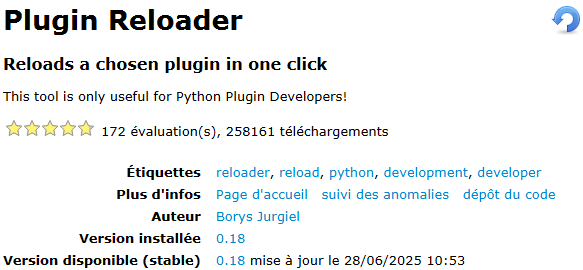
\includegraphics[width=0.75\linewidth]{5_develloppeur/fig/plugin_reloader.png}
    \caption{Description sheet for \script{Plugin Reloader}}
    \label{fig_plugin_reloader}
\end{figure}

\subsection{The QGIS plugin \script{First Aid}}

The \script{First Aid} plugin allows investigating errors occurring during plugin execution. 


\newpage
\subsection{VS-Code}
The \script{debugvs} plugin allows connecting a \script{VS-Code} debugging instance to the plugin execution from QGIS. This debugging configuration allows using all VS Code features during debugging (breakpoints, watch, call stack...). Setting up this debugging configuration is done as follows: 
\begin{enumerate}
    \item install \script{debugpy} with the command \script{!pip install debugpy} from the QGIS Python command prompt;
    \item \sloppy if the plugin development directory is not located in \texttt{C://Users/$USER$/AppData//QGIS/QGIS3/profiles/default/python}, create a symbolic link in this directory pointing to the development directory.  
    \item install the \script{debugvs} plugin by downloading its script from the GitLab repository \url{https://github.com/lmotta/debug_vs} and activate the plugin by importing the \script{.zip} folder in \script{QGIS} (\cffig \ref{fig_debugvs}); 
    \begin{figure}[H]
        \centering
        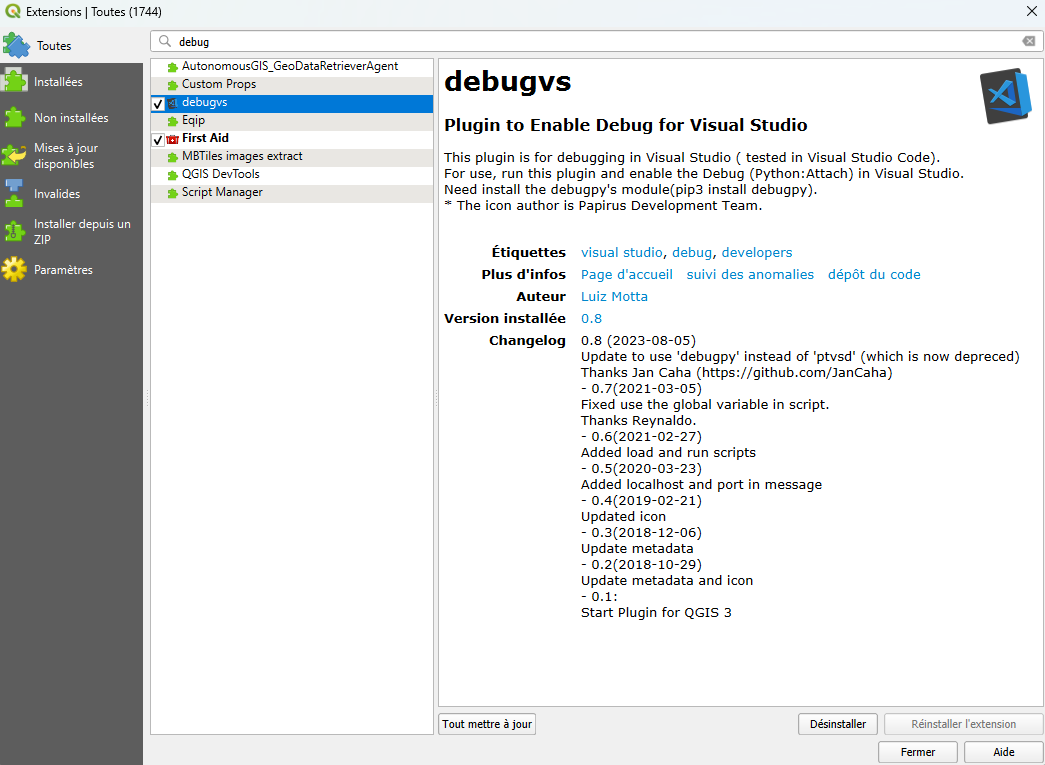
\includegraphics[width=0.6\linewidth]{5_develloppeur/fig/debugvs.png}
        \caption{\script{debugvs} plugin}
        \label{fig_debugvs}
    \end{figure}
    \item configure VS Code to connect to QGIS during a debugging session: 
    \begin{enumerate}
        \item in the CaWaQS-Viz development directory, create a \script{.vscode} sub-directory (add this directory to the \script{.gitignore} file); 
        \item create a \script{settings.json} file in the \script{.vscode} sub-directory and copy the content from code \ref{code_settings_vscode}. Optionally modify the directory paths to match your QGIS and Python installation and operating system. This one is for Windows.
        \begin{lstlisting}[language=JSON, caption={Workspace configuration file. This file defines the Visual Studio Code workspace configuration for QGIS plugin development. It adapts the VS Code Python environment to that used by QGIS (installed via OSGeo4W).}, label=code_settings_vscode]
        {   
            
            "workbench.colorCustomizations": {
                "titleBar.activeBackground": "#006823",
                "editor.background": "#000000"
            },
            
            "python.linting.pylintEnabled": true,
            "python.jediEnabled": true,
        
            
            "python.pythonPath": "C:/OSGeo4W64/bin/python-qgis.bat",
        
        
            "python.linting.pylintArgs": [
                "--extension-pkg-whitelist=PyQt5,qgis,db_manager",
                "--disable=all",
                "--enable=F,E,unreachable,duplicate-key,unnecessary-semicolon,global-variable-not-assigned,unused-variable,binary-op-exception,bad-format-string,anomalous-backslash-in-string,bad-open-mode"
            ],
        
           
            "terminal.integrated.env.windows": {
                
                "PATH": "C:\\OSGeo4W\\apps\\qgis\\bin;C:\\OSGeo4W\\apps\\Python312;C:\\OSGeo4W\\apps\\Python312\\Scripts;C:\\OSGeo4W\\apps\\Qt5\\bin;C:\\OSGeo4W\\apps\\Python312\\Scripts;C:\\OSGeo4W\\bin;C:\\Windows\\System32;C:\\Windows;C:\\Windows\\system32\\WBem;C:\\OSGeo4W\\apps\\Python312\\lib\\site-packages\\pywin32_system32;C:\\OSGeo4W\\apps\\Python312\\lib\\site-packages\\numpy\\.libs",
                
                "PYTHONHOME": "C:\\OSGeo4W\\apps\\Python312",
                "PYTHONPATH": "C:\\OSGeo4W\\apps\\qgis\\python;%PYTHONPATH%",
                
                "GDAL_DATA": "C:\\OSGeo4W\\share\\gdal",
                "GDAL_DRIVER_PATH": "C:\\OSGeo4W\\bin\\gdalplugins",
                "GDAL_FILENAME_IS_UTF8": "YES",
                
                "GEOTIFF_CSV": "C:\\OSGeo4W\\share\\epsg_csv",
                
                "O4W_QT_BINARIES": "C:/OSGeo4W/apps/Qt5/bin",
                "O4W_QT_DOC": "C:/OSGeo4W/apps/Qt5/doc",
                "O4W_QT_HEADERS": "C:/OSGeo4W/apps/Qt5/include",
                "O4W_QT_LIBRARIES": "C:/OSGeo4W/apps/Qt5/lib",
                "O4W_QT_PLUGINS": "C:/OSGeo4W/apps/Qt5/plugins",
                "O4W_QT_PREFIX": "C:/OSGeo4W/apps/Qt5",
                "O4W_QT_TRANSLATIONS": "C:/OSGeo4W/apps/Qt5/translations",
                "QT_PLUGIN_PATH": "C:\\OSGeo4W\\apps\\qgis\\qtplugins;C:\\OSGeo4W\\apps\\Qt5\\plugins",
                
                "QGIS_PREFIX_PATH": "C:/OSGeo4W/apps/qgis",
                
                "VSI_CACHE": "TRUE",
                "VSI_CACHE_SIZE": "1000000"
            },
            "python.languageServer": "Jedi", 
        }
\end{lstlisting} 
        \item create a \script{launch.json} file in the \script{.vscode} sub-directory, copy the content from code \ref{code_launch_vscode}, modify the \script{localRoot} and \script{remoteRoot} paths to match your workspace configuration.
        
        \begin{lstlisting}[language=JSON, caption={VS-Code debugger configuration file. In this configuration, the "connect" section indicates the address and port on which QGIS exposes the debugging session (here localhost:5678). The "pathMappings" block establishes the correspondence between the local project paths open in VS Code (localRoot) and the paths used by QGIS to execute the plugin (remoteRoot). This correspondence is essential for breakpoints placed in VS Code to be correctly associated with the files actually executed by QGIS.}, label = code_launch_vscode]
{
    "version": "0.2.0",
    "configurations": [
        {
            "name": "Attach QGIS Debug",
            "type": "python",
            "request": "attach",
            "connect": {
                "host": "localhost",
                "port": 5678
            },
            "pathMappings": [
                {
                    "localRoot": "C:\\Program Files\\$QGIS$\\apps\\qgis-ltr\\python\\plugins\\cawaqsviz",
                    "remoteRoot": "C:\\Users\\$USER$\\AppData\\Roaming\\QGIS\\QGIS3\\profiles\\default\\python\\cawaqsviz"
                }
            ],
            "justMyCode": false
        }
    ]
}


\end{lstlisting}
        \end{enumerate}
    \item Establish the QGIS/VS-Code connection
    \begin{enumerate}
        \item authorise the debugger connection to QGIS via the \script{debugvs} plugin (\cffig \ref{fig_enable_vscode_qgis});
        \begin{figure}[H] 
            \centering
            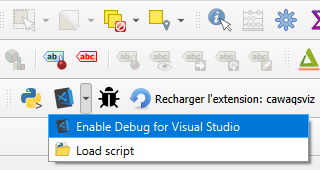
\includegraphics[width=0.40\linewidth]{5_develloppeur/fig/launch_debug_vs.png}
            \caption{Establishing a QGIS/VS-Code connection from the \script{debugvs} plugin}
            \label{fig_enable_vscode_qgis}
        \end{figure}
        \item launch the VS-Code debugging session (\cffig \ref{fig_debug_VS_CODE}).
        \begin{figure}[H]
            \centering
            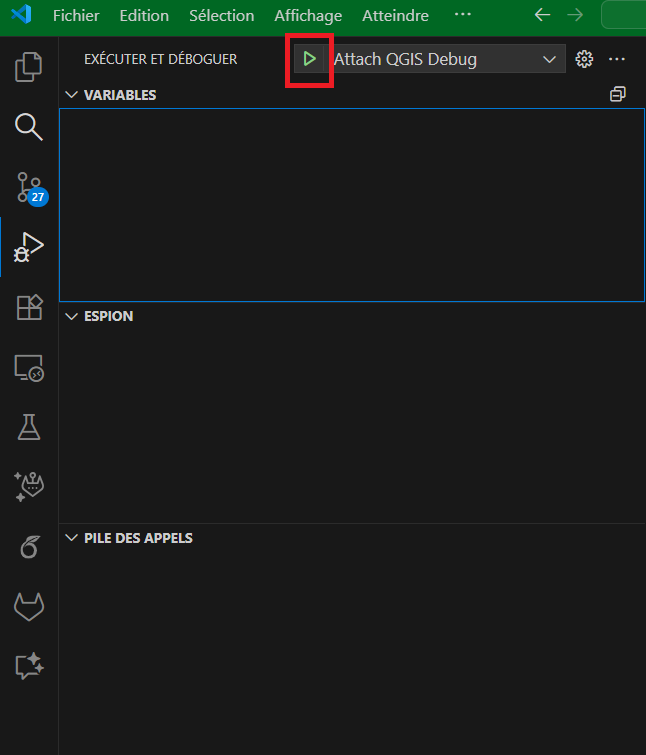
\includegraphics[width=0.5\linewidth]{5_develloppeur/fig/debug_vs_code.png}
            \caption{Launching a debugging session from VS-Code}
            \label{fig_debug_VS_CODE}
        \end{figure}
    \end{enumerate}
\end{enumerate} 

The connection between the debugger and QGIS is terminated from VS-Code by clicking on \script{"Disconnected"} in the debugging toolbar (\cffig \ref{fig_barre_outil_debbug}) 

\begin{figure}[H]
    \centering
    
\includegraphics[width=0.35\linewidth]{5_develloppeur/fig/disconnect-debugger.png}
    \caption{VS-Code debugger toolbar}
    \label{fig_barre_outil_debbug}
\end{figure}




\newpage
\section{Creating Dialog Boxes with \script{Qt Designer}} 
\ref{sec_QtDesigner}
The \script{Qt Designer} application, provided with the QGIS installation (installation with OSGEO), is a tool for creating dialog boxes in the form of .ui files. In the \cwv~application, all dialog boxes have their own \script{.py} file to which the \script{.ui} file, of the same name, is associated with the dialog box's Python class. 

\begin{lstlisting}[language = Python, label = code_init_from_ui, caption = Initialisation of the "Compare SIM/OBS" dialog box from a .ui file]
# This loads your .ui file so that PyQt can populate your plugin with the elements from Qt Designer
FORM_CLASS, _ = uic.loadUiType(
    os.path.join(os.path.dirname(__file__), "DialogComparesimobs.ui")
)


class DialogComparesimobs(Dialog, FORM_CLASS):
    def __init__(self, iface:QgisInterface, log_file_path:str, parent=None):
        """Constructor Method

        :param iface: Qgis Interface
        :type iface: QgisInterface
        :param logFilePath: Path of the cawaqs-viz log file, defaults to None
        :type logFilePath: str, optional
        :param parent: Parent class, defaults to None
        :type parent: _type_, optional
        """
        super(DialogComparesimobs, self).__init__(parent)
        self.setupUi(self)
        self.iface = iface
        self.logFilePath = log_file_path
        self.simData = False
\end{lstlisting}

\newpage
\section{Manual Plugin Configuration for developers}
\label{sec-config-manual}

The lower part of the \gui{Settings} dialog box allows manual configuration
of the plug-in. The following elements must be defined:
\begin{enumerate}
    \item a project name;

    \item the modelled compartments;

    \item a GIS layer mesh configuration;

    \item the modelling output and observation directories\footnote{The flow and piezometry observation directories are assumed to be in the same parent directory.} if observation points are defined in the project.
\end{enumerate}

The project name will be used to name a sub-folder created in the post-processing directory. The graphical outputs of the \cwv~application will be placed
in this post-processing folder.\\

The geometry configuration can also be imported from a \json~configuration file (by clicking on \gui{Import a geometry configuration from a \json})
or defined manually \textit{via} the option \gui{Select resolutions from the current project}.

\alertinfo{Note that any manual project and geometry configuration will be exported in \json~format to the post-processing directory upon execution of the \gui{Settings} dialog box.}

\subsection{Contents of the QGIS Project Used for Processing \cawaqs~Simulation Results}
\label{sec-res-cawaqs}

\textbf{{The \script{shapefiles} of the \cawaqs~model meshes}}\\
The QGIS project used for processing simulations with the \cwv~utility
must contain:
\begin{itemize}
    \item the meshes (resolutions) of the compartments in \gui{shapefile}
        format of the model (refer to the \cawaqs~documentation\footnote{\cawaqs~geometry terminology. For more information on the different types of meshes,
        refer to the model documentation (\ie~user guide and technical guide),
        available on the GitLab repository \href{https://gitlab.com/cawaqs/cawaqs}{https://gitlab.com/cawaqs/cawaqs}.}
        to identify the output resolutions of the \gui{WATBAL} compartment).
        The \cawaqs~resolution types to import into the GIS project for
        processing modelling outputs depend on the compartments
        actually being modelled;

    \item the observation points of the compartments to be defined in the \cwv~extension.
\end{itemize}

\begin{table}[H]
    \centering
    \begin{tabular}{>{\raggedleft\arraybackslash}m{3cm}|>{\centering\arraybackslash}m{3.2cm}>{\centering\arraybackslash}m{3.2cm}>{\centering\arraybackslash}m{3.2cm}>{\centering\arraybackslash}m{3.2cm}}
        \hline
                                                                & \textbf{Surface compartment\newline(WATBAL)}                                                               & \textbf{Hydraulic compartment \newline(HYD)} & \textbf{Unsaturated compartment \newline(NSAT)} & \textbf{Aquifer compartment \newline(AQ)} \\
        \hline
        \textbf{\cawaqs~resolution}                             & Unit surface cell (\texttt{ele\_bu})\footnotemark~ \newline or Production cell (\texttt{Cprod}) & River element (\texttt{ele\_musk})            & Unsaturated zone grid                     & Meshes of all aquifer layers   \\
        \hline
        \textbf{Required fields in the attribute table} & Cell identifiers                                                                                      & GIS identifiers of river elements          & Cell identifiers                        & Absolute cell identifiers            \\
        \hline
    \end{tabular}
    \caption{\cawaqs~resolutions that can be imported as compartment resolution.}
    \label{tab-resolution_per_compartment}
\end{table}

\alertwarning{The names of the GIS layers in the project corresponding to aquifers must be identical to those defined in the CaWaQS configuration to ensure correct application behaviour.}

\textbf{{The \script{shapefiles} of extraction points}}\\

Extraction of simulated flow and hydraulic head can be performed at
extraction points. Two types of extraction points can be
defined:
\begin{itemize}
    \item simple extraction points, which do not include a measurement
        time series;

    \item observation points, which are extraction points with measurement
        data.
\end{itemize}

Extraction and observation points are contained in two separate
\script{shapefile} files whose attribute tables contain the fields
listed in table \ref{tab_obs_extract}.

\vspace{8pt}

\renewcommand{\arraystretch}{1.5} % to add spacing between rows
\newcolumntype{C}[1]{>{\centering\arraybackslash}p{#1}} \newcolumntype{C}[1]{>{\centering\arraybackslash}p{#1}}

\begin{table}[H]
    \begin{tabular}{|C{0.2\textwidth}|C{0.35\textwidth}|C{0.35\textwidth}|}
        \hline
        \textbf{POINT TYPE}& \textbf{ATTRIBUTE TABLE CONTENTS} & \textbf{OUTPUTS} \tabularnewline                    \hline
        \textbf{Extraction point}  & 
        \begin{itemize}[leftmargin=*, itemsep=0.5ex]
            \item Point name
            \item Identifier of the attached cell\footnote{\gui{GIS ID} if extraction in the HYD compartment, \gui{ABS ID} if extraction in aquifer, optional field}, aquifer layer identifier (if extraction in aquifer)\end{itemize} & \begin{itemize}[leftmargin=*, itemsep=0.5ex]\item Simulated hydrographs and piezometric curves at the extraction point\end{itemize} \tabularnewline                     \hline
        \textbf{Observation point} & 
        \begin{itemize}[leftmargin=*, itemsep=0.5ex]
            \item Point name
            \item Identifier of the attached cell \footnotemark[\value{footnote}]
        \end{itemize} & 
        \begin{itemize}[leftmargin=*, itemsep=0.5ex]
            \item Simulated and observed hydrographs and piezometric curves
            \item Objective criteria comparing observations with simulations
        \end{itemize} \tabularnewline \hline
    \end{tabular}
    \label{tab_obs_extract}
    \caption{Structure of GIS layers for extraction points and associated graphical outputs}
\end{table}

\vspace{8pt}

\alertwarning{Observation \script{shapefiles} must be imported into the project and specified in the \cwv~configuration if the HYD and/or AQ compartments are being processed. Without observations, the extension will not be functional.}

\subsection{Configuring the Project Geometry from an Existing QGIS Project}
\label{sec_config_manuelle}

The geometric configuration of the \cwv~application can be defined from an existing QGIS project via the \gui{Application configuration from an existing project}
dialog box in the application settings dialog.

The window is organised into two sections:
\begin{itemize}
    \item on the left, the \cawaqs~compartments are listed (WATBAL, HYD, AQ,
        NSAT),

    \item on the right, the parameters to be defined are listed for producing
        graphical outputs (flow and piezometry) at observation points
        (extraction points with observations) or extraction points (without observations).
\end{itemize}

If the application configuration fields are left empty, the
compartment concerned is not included in the geometric configuration.\\

The compartment fields are configured as follows:\\

\noindent
\textbf{The surface compartment (\gui{"WATBAL COMPARTMENT"}) :}

\vspace{0.5em}

\begin{minipage}[t]{0.45\textwidth}
    \begin{itemize}
        \item \gui{Surface resolution}: output resolution of the surface water balance (CPROD or elebu);
        \item \gui{cell id}: the column number in the attribute table corresponding to the cell identifier;
        \item \gui{cell area}: the column number in the attribute table corresponding to the cell area (optional parameter).
    \end{itemize}
\end{minipage}%
\hfill
\begin{minipage}[t]{0.45\textwidth}
    \centering
    \raisebox{\dimexpr-\height+\ht\strutbox}{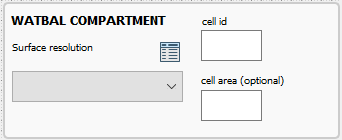
\includegraphics[
        width=0.8\linewidth
    ]{
        2_application_user_guide/fig/DialogSelectLayer_watbal.png
    }} \captionof{figure}{WATBAL compartment configuration fields}
\end{minipage}

\vspace{1em}
\textbf{The hydraulic compartment (\gui{HYD COMPARTMENT})}

\begin{minipage}[t]{0.45\textwidth}
    \begin{itemize}
        \item \gui{Hyd resolution}: name of the output resolution of the \gui{HYD} compartment (river elements);
        \item \gui{GIS Id}: the column number in the attribute table corresponding to the GIS identifier of the cells 
    \end{itemize}
\end{minipage}%
\hfill
\begin{minipage}[t]{0.45\textwidth}
    \centering
    \raisebox{\dimexpr-\height+\ht\strutbox}{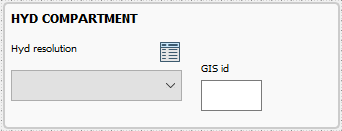
\includegraphics[
        width=0.8\linewidth
    ]{
    2_application_user_guide/fig/DialogSelectLayer_hyd.png
    }} 
    \captionof{figure}{HYD compartment configuration fields}
\end{minipage}

\vspace{1em}
\textbf{The unsaturated compartment (\gui{NSAT COMPARTMENT}):}

\begin{minipage}[t]{0.45\textwidth}
    \begin{itemize}
        \item \gui{Unsatured zone resolution}: name of the output resolution of the \gui{NSAT} compartment;
        \item \gui{cell id}: the column number in the attribute table corresponding to the cell identifier. 
    \end{itemize}
\end{minipage}%
\hfill
\begin{minipage}[t]{0.45\textwidth}
    \centering
    \raisebox{\dimexpr-\height+\ht\strutbox}{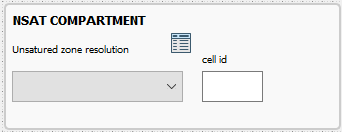
\includegraphics[
        width=0.8\linewidth
    ]{
    2_application_user_guide/fig/DialogSelectLayer_nsat.png
    }} 
    \captionof{figure}{NSAT compartment configuration fields}
\end{minipage}

\vspace{1em}
\textbf{The saturated compartment (\gui{AQ COMPARTMENT})}

\begin{minipage}[t]{0.45\textwidth}
     \begin{itemize}
            \item \gui{Aquiferes resolutions}: the GIS layers constituting the
                underground mesh. The selected layer is added by clicking
                on \gui{Add}. Layers must be ordered from the uppermost
                to the lowermost layer using the \gui{up} and \gui{down} buttons.
                Finally, a layer can be removed from the list by clicking on
                \gui{remove};
            \item \gui{cell id abs}: identifier of the attribute table column
                containing the absolute cell identifier. This identifier
                can be homogeneous across GIS layers: in that case, \gui{homogeneous ID ABS}
                must be selected. Otherwise, click on \gui{heterogeneous ID ABS}
                to open dialog boxes allowing you to specify, for
                each layer, the column containing the ABS ID of the cells (cf. Fig \ref{fig_id_abs_hetero}).
        \end{itemize}
\end{minipage}%
\hfill
\begin{minipage}[t]{0.45\textwidth}
    \centering
    \raisebox{\dimexpr-\height+\ht\strutbox}{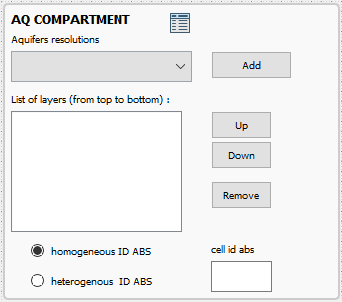
\includegraphics[
        width=0.8\linewidth
    ]{
    2_application_user_guide/fig/DialogSelectLayer_aq.png
    }} 
    \captionof{figure}{AQ compartment configuration fields}
    \raisebox{\dimexpr-\height+\ht\strutbox}{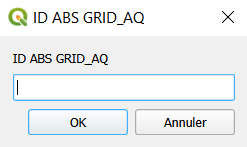
\includegraphics[
        width=0.5\linewidth
    ]{
2_application_user_guide/fig/DialogSelect_Layer_hetero_ID_ABS
    }} 
    \label{fig_id_abs_hetero}
    \captionof{figure}{Window for selecting the field identifier containing the \gui{ID ABS} in the attribute table in the case of heterogeneous field identifiers across layers}
\end{minipage}



\alertwarning{Some points of caution:}
\begin{itemize}
    \item \textbf{The identifier of the first column of an attribute table starts at 0}. The icon 
\includegraphics[height=0.45cm]{2_application_user_guide/fig/table.png} allows viewing the identifiers of the fields listed in the attribute table of the resolution selected in the drop-down list;
    \item the code (e.g., BSS code) of an observation point must be \textbf{unique} among all observation points;
    \item The geometric configuration of the compartments checked in the project parameterisation dialog box must be defined in the geometry configuration dialog box.
\end{itemize}

\vspace{8pt}

\textbf{Extraction points - \gui{Hydrological and Hydrological plots}} \\
Extraction points can be of two types:
\begin{itemize}
    \item[$\bullet$] simple extraction points, which allow
    viewing simulated variables at those points;
    \item[$\bullet$] observation points, which allow comparing simulated variables with observation data at those points.
\end{itemize}



The configuration of extraction points requires specifying in the \gui{GIS Layer} fields the name of the layer in the QGIS project containing the observation points and extraction points according to the relevant \cws~compartment. The field identifiers to be specified are as follows: 
\vspace{8pt}

\begin{minipage}[t]{0.45\textwidth}
    \textbf{Extraction points of the \gui{HYD} compartment} 
    \vspace{4pt}

     \underline{Extraction points}

    \begin{itemize}
        \item \gui{name}: name of the observation point;
        \item \gui{ID GIS}: GIS identifier of the observation point to which the observation point must be attached (optional field)
    \end{itemize}

    \vspace{2pt}
    \underline{Observation points} 
    \begin{itemize}
        \item \gui{code}: identification code of the observation point, must be unique for each point. The observation file for the point must have the same name with the \script{.dat} extension;
        \item the \gui{name} and \gui{ID GIS} fields are also specified for the configuration of observation points 
    \end{itemize}
    \vspace{8pt}
    \textbf{Extraction points of the \gui{AQ} compartment} 
    \vspace{4pt}

     \underline{Extraction points}

    \begin{itemize}
        \item \gui{name}: name of the observation point;
        \item \gui{ID LAYER}: identifier of the aquifer layer
        \item \gui{ID GIS}: GIS identifier of the observation point to which the observation point must be attached (optional field)
    \end{itemize}

    \vspace{2pt}
    \underline{Observation points} 
    \begin{itemize}
        \item \gui{code}: identification code of the observation point, must be unique for each point. The observation file for the point must have the same name with the \script{.dat} extension;
        \item the \gui{name} and \gui{ID GIS} fields are also specified for the configuration of observation points
    \end{itemize}

    
\end{minipage}%
\hfill
\begin{minipage}[t]{0.45\textwidth}
    \centering
    \raisebox{\dimexpr-\height+\ht\strutbox}{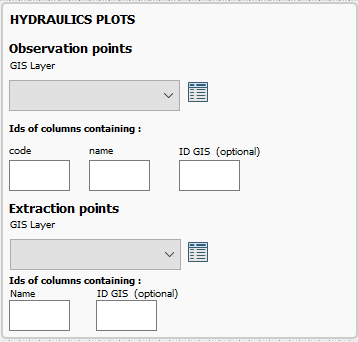
\includegraphics[
        width=0.9\linewidth
    ]{
    2_application_user_guide/fig/DialogSelectLayer_hyd_extraction.png
    }} 
    \captionof{figure}{Configuration fields for \gui{HYD} compartment extraction points}
    \vspace{4pt}
    \raisebox{\dimexpr-\height+\ht\strutbox}{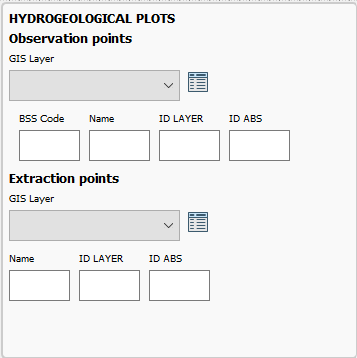
\includegraphics[
        width=0.9\linewidth
    ]{
    2_application_user_guide/fig/DialogSelectLayer_aq_extraction
    }} 
    \label{fig_id_abs_hetero}
    \captionof{figure}{Configuration fields for \gui{AQ} compartment extraction points}
\end{minipage}

\alertwarning{
Extraction points must be contained in a \script{.shp} file different from the observation points. Points cannot be contained in the same file if they are extracted from two different compartments.
}


\alertinfo{
A preliminary save of the geometry configuration file can be saved by specifying a file path in the field located at the bottom left of the dialog box. This file (\cfcod \ref{code_config_geom}) will be saved upon execution of the \gui{Settings} dialog box if the configured project does not yet exist in the post-processing
directory specified. 
Multiple project configurations can be saved in the same post-processing directory, provided they do not have the same project name. }



\subsection{Configuring Resolutions from a \json~Configuration File}

The geometric configuration of resolutions can be specified via a
\json~file according to the following structure:

\begin{lstlisting}[language=json, caption={Contents of a geometry configuration file}, label={code_config_geom}]
{   // list of CaWaQS compartments to analyse (1 = AQ, 2 = HYD, 3 = WATBAL) 
    "ids_compartment": [], 
                           
    "resolutionNames": 
    {
        "1": 
            [[""]], // list of names of aquifer meshes in the QGIS project 
        "2" : 
            [[""]], // name of the river mesh in the QGIS project 
        "3" : 
            [[""]] // name of the surface mesh in the QGIS project 
        "4" : 
            [[""]] // name of the unsaturated zone mesh in the QGIS project 
        }, 
    "ids_col_cell": { // "compartment id" : "column number of cell id"
        "1" : "",  // "AQ id" : "absolute id column number"
        "2" : "",  //"HYD id" : "GIS id column number"
        "3" : ""   // "WATBAL id" : "cell id column number"
        }, 
    "obsNames": { 
    // "compartment id" : "name of associated obs shp in the QGIS project"
        "1": "", 
        "2" : ""
        }, 
    "obsIdsColCells": {
    // "compartment id" : "field number of the measurement point code"
        "1": "", 
        "2": ""
        }, 
    "obsIdsColNames": { 
    // "compartment id" : "field number of the measurement point name"
        "1": "", 
        "2" : ""
        }, 
    "obsIdsColLayers": { 
    // "compartment id" : "field number of the aquifer layer identifier"
        "1": "", 
        "2" : null
        }, 
    "obsIdsCell": { 
    // "comp. id" : "field number of the absolute or gis id of cell attached to obs"
        "1" : "", 
        "2" : null
    }, 
     "extNames": {
    // "compartment id" : "name of associated extraction shp in the QGIS project"
        "2": "",
        "1": ""
    },
    "extIdsColNames": {
    // "compartment id" : "field number containing the extraction point name"
        "2": "",
        "1": ""
    },
    "extIdsColLayers": {
    // "compartment id" : "field number containing the aquifer layer identifier"
        "2": null,
        "1": ""
    },
    "extIdsColCells": {
    // "compartment id" : "field number containing the cell identifier"
        "1": "",
        "2": "",
    }
}
}
\end{lstlisting}

